\documentclass[a4paper]{article}

\input ../header
\usepackage[np]{numprint}

\setlength{\multicolsep}{2pt}

\begin{document}

\title{Sujet B -- Internet}

\pagestyle{empty}

\date{}
\author{}

\maketitle{}
\thispagestyle{empty}

% Petit exercice de conversion, rappels
\exo[2 points]\vspace*{-2mm}
\begin{enumerate}
  \item Qu'est-ce qu'un octet ?\rep{4}
  \item Convertir la quantité $50$ Mb (mégabits) en Mo (mégaoctets) puis en Go (gigaoctets).\rep{4}
\end{enumerate}

\bigskip

% Exercice définitions
\exo[1 point] Relier chaque mot à la bonne définition :

\begin{center}
  \begin{tabular}{@{}r@{\hspace{4cm}}l@{}}
    Mosaic $\bullet$ & $\bullet$ service qui permet de traduire\\
		  & \phantom{$\bullet$} un nom de domaine en adresse IP\\
		  &\\
    Arpanet $\bullet$ & $\bullet$ un des premiers navigateurs web\\
		       &\\
    Cyclades $\bullet$ & $\bullet$ projet expérimental français ayant pour\\
		      & \phantom{$\bullet$} but de créer un réseau d'ordinateurs\\
		      &\\
    DNS $\bullet$ & $\bullet$ premier réseau à transfert\\
		     & \phantom{$\bullet$} de paquets développé aux États-Unis\\
  \end{tabular}
\end{center}

\bigskip

\exo[1 point] Donner le nom d'un câble sous-marin arrivant en Polynésie.\rep{3}

\bigskip

% Temps de téléchargement d'un fichier avec un forfait Fibre
\exo[4 points]\vspace*{-2mm}
Chez lui, Arii dispose d'une connexion Vinibox SPRINT :

\begin{center}
  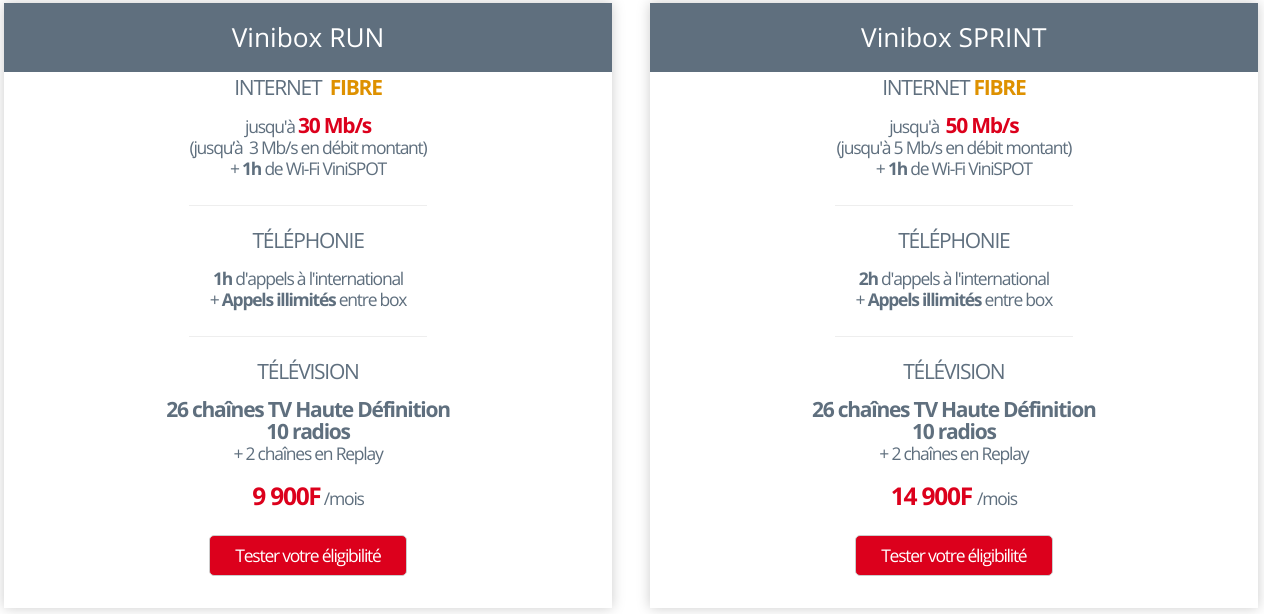
\includegraphics[width=15cm]{evaluation_2_seconde_15_sujet_B_offres_vinibox_fibre.png}
\end{center}

\begin{enumerate}
  \item Hawaiiki demande à Arii de lui télécharger une version de son film favori, \textit{Drive}. Combien de temps prendra le téléchargement, sachant que le fichier souhaité occupe $2,1$ Go ? (on supposera qu'Arii le télécharge à la vitesse maximale théorique annoncée par son fournisseur d'accès)\rep{10}
  \item Heitea souhaite ardemment aider Hawaiiki : elle aussi se met à télécharger le film. Sachant que Heitea peut télécharger à la vitesse de $4$ Mo par seconde, combien de temps mettra-t-elle ?\rep{10}
\end{enumerate}

\bigskip

% Comparaison avec ADSL
\exo[2 points] Expliquer la durée annoncée de téléchargement d'un jeu vidéo de $25$ Go sur la capture d'écran ci-dessous :

\begin{center}
  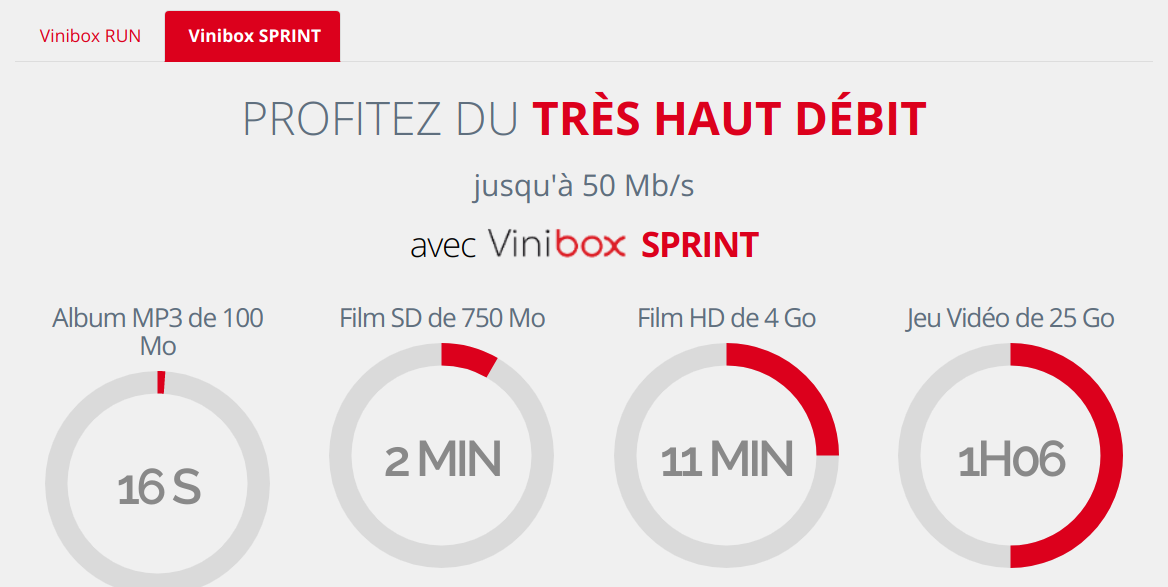
\includegraphics[width=15cm]{evaluation_2_seconde_15_sujet_B_vini.png}
\end{center}

\dotfill\rep{9}

\end{document}
